\documentclass[main.tex]{subfiles}
\begin{document}

\section*{Mon Nov 04 2019}

% No lectures tomorrow, instead on Wednesday at 14.30.

\subsection{Isothermal winds with an external force}

Last time we found that the only physical solution to the stellar wind is the transsonic solution.

Now, let us add an external force:


%
\begin{align}
  v \dv{v}{r} = - \frac{1}{\rho } \dv{P}{r} - \frac{GM}{r^2} + f(r)
\,,
\end{align}
%
so we get 
%
\begin{align}
  \frac{1}{v} \dv{v}{r} = \frac{2 \frac{a^2}{r} - \frac{GM}{r^2} + f(r)}{v^2 - a^2}
\,,
\end{align}
%
with the speed of sound \(a = \sqrt{\mathcal{R} T / \mu } \). How does the velocity gradient change?
With an outward force, we expect the velocity gradient to be less steep in the subsonic region (the velocity decreases slower: the numerator is \emph{less negative}).
Adding this force is formally equivalent to modifying the gravitational field by making it weaker. This increases the pressure scale height, so the density gradient becomes less steep, so the velocity gradient becomes less steep as well.

In the supersonic region, instead the gradient will be larger: the numerator is \emph{more positive} and higher velocities are reached.

The critical radius changes: it is the solution to 
%
\begin{align}
  r_C = \frac{GM}{2 a^2} - \frac{f(r_C) r_C^2}{2 a^2}
\,,
\end{align}
%
which will shift inward as \(f\) goes from 0 to positive.
This is shown in figure \ref{fig:critical_radius_position}.

\begin{figure}[H]
\centering
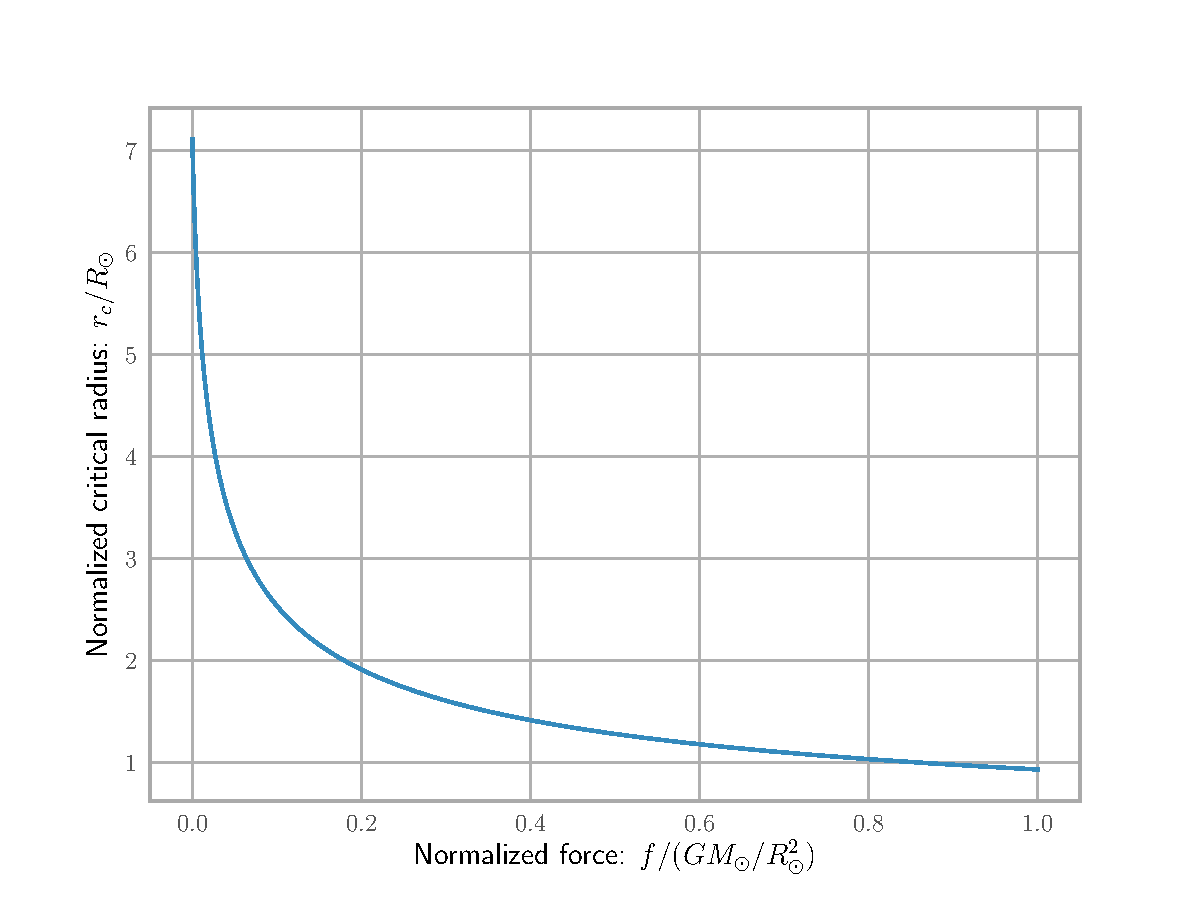
\includegraphics[width=\textwidth]{figures/critical_radius_position.pdf}
\caption{Critical radius position in function of a constant force, expressed in units of the gravitational acceleration at the surface. Here, we assume solar parameters and \(T = \SI{e6}{K}\).}
\label{fig:critical_radius_position}
\end{figure}

The adiabatic speed of sound is the same, it does not depend on \(f\). Also, the velocity gradient is less steep as we said before. 
These two facts combined mean that the velocity at the corona, \(v_0 \), must be larger.

Since \(\rho' / \rho + v' / v + 2/r = 0\), and the critical radius velocity is \(v=a\) regardless of the value of \(f\), and the critical radius decreases if we have \(f>0\), we must have that \(\rho_{c}\), the density at the critical radius, must be smaller than that with \(f=0\).

How do we expect the mass loss rate to change? from the continuity equation at the bottom of the corona, we get \(\dot{M} = 4 \pi r_0^2 \rho_0 v_0 \), and everything on the RHS is fixed but \(v_0 \), so when we increase \(f\) the LHS must incrase as well. 

Let us consider some explicit law scaling as \(f \propto r^{-2}\), like a radiative force: 
%
\begin{align}
  g _{\text{rad}} \propto \kappa_F  \times \qty(\frac{r}{R})^{-2}
\,.
\end{align}

This is the same as changing the mass of the star, since it scales like the gravitational force. We then take our force to be \(f(r) = A / r^2\). Our momentum equation, with the pressure gradient substituted in from the differentiated ideal gas law and the continuity equation, becomes
%
\begin{align}
  \frac{1}{v} \dv{v}{r}  = \qty(\frac{2 a^2}{r} - \frac{GM}{r^2} + \frac{A}{r^2}) / \qty(v^2- a^2)
\,,
\end{align}
%
which is the same as the equation without force, with a smaller effective mass:
\(M _{\text{eff}} = M ( 1- A / GM)\).

The correction is usually called the Eddington ratio: 
%
\begin{align}
  \Gamma = \frac{A}{GM} = \frac{A/r^2}{GM / r^2}
\,,
\end{align}
%
the acceleration of the force divided by the gravitational one.

% \todo[inline]{Are the units of \(A\) and \(GM\) not \SI{}{m^3 s^{-2}}?}

If \(A\) is a consant, the critical radius becomes 
%
\begin{align}
  r_C = \frac{GM}{2a^2} \qty(1 - \Gamma )
\,,
\end{align}
%
however in general \(A\) is not taken as a constant, instead it is modelled with a Heaviside theta function, so that it only activates after a certain radius.

As \(\Gamma \) increases, the critical velocity is reached faster, and the velocity at the corona is greater.
The density profile gets less and less steep: the density scale height decreases.

We approximate \(A(r) = A [r \geq r_d]\) for some \(r_d\).\footnote{Using the Iverson bracket here!}
The justification for this model is that below the dust condensation region there is only gas, above it there is dust which is more opaque to radiation.
We are still assuming the wind is isothermal.

The critical point depends on \(\Gamma \): 
%
\begin{align}
  \frac{r_C}{1 - \Gamma (r_C)} = \frac{GM}{2 a^2}
\,.
\end{align}
%

If the extra force switches on \emph{outside} the critical region, the mass loss rate is \emph{unchanged}, since it only depends on the subsonic region.

\todo[inline]{Is there the possibility to have more than one critical radius with only outward force?}

There is a maximum value of \(\Gamma\) such that the critical radius \(r_C\) is equal to the radius of the star. 

As \(\Gamma \) increases towards this value, the mass loss rate increases greatly. 
If \(\Gamma \) is larger than this value, and \(v_0 \) is subsonic, then the RHS of the momentum equation is \emph{negative}: the velocity gradient is negative, the velocity decreases. 

\end{document}